\subsection{Metodo del Gradiente}
Il metodo del gradiente è un algoritmo che calcola il vettore di minimo globale, ovvero:
Un vettore $x^{\ast}$ è un punto di minimo globale di $f(x)$ se $f(x^{\ast}) \leq f(x) \forall x \in R^n$.

Analogamente, un vettore $x^{\ast}$ è un punto di minimo globale in senso stretto di $f(x)$ 
se $f(x^{\ast}) < f(x) \forall x \in R+n \and x \neq x^{\ast}$.

\begin{figure}[H]
    \centering
    \begin{subfigure}{0.9\textwidth}
        \centering
    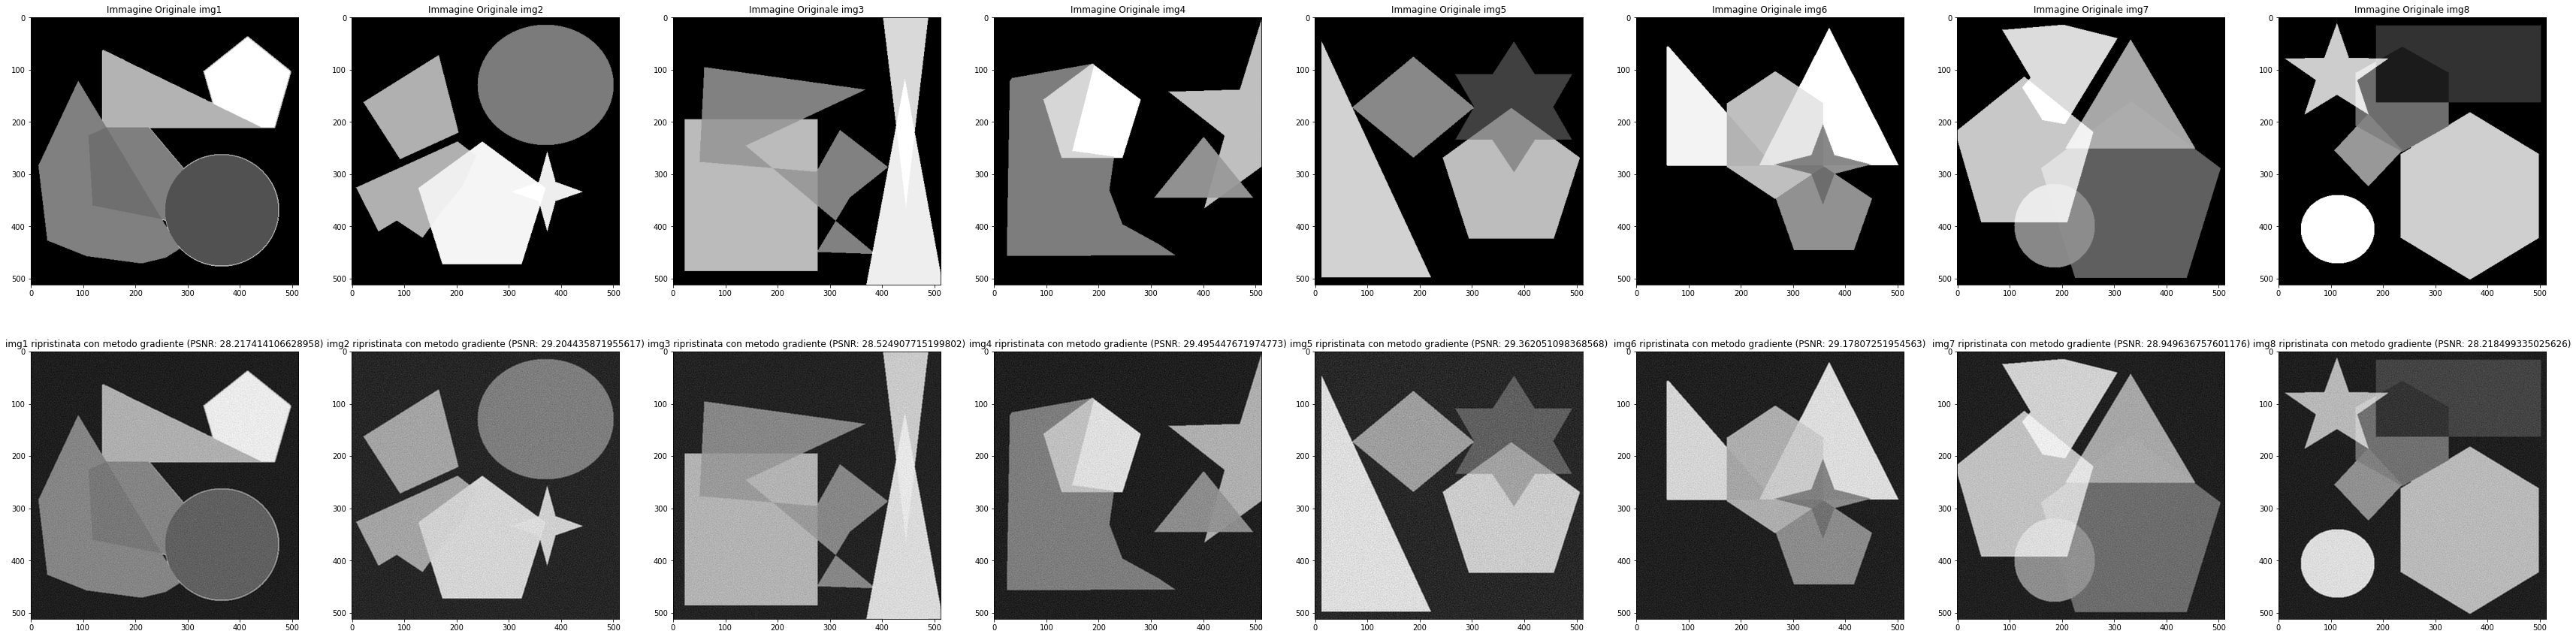
\includegraphics[width=0.7\textwidth]{imgRel/datasetgradiente.png}\label{fig:geomgradiente}
    \caption{Immagini geometriche ripristinate}
    \end{subfigure}

    \begin{subfigure}{0.5\textwidth}
        \centering
        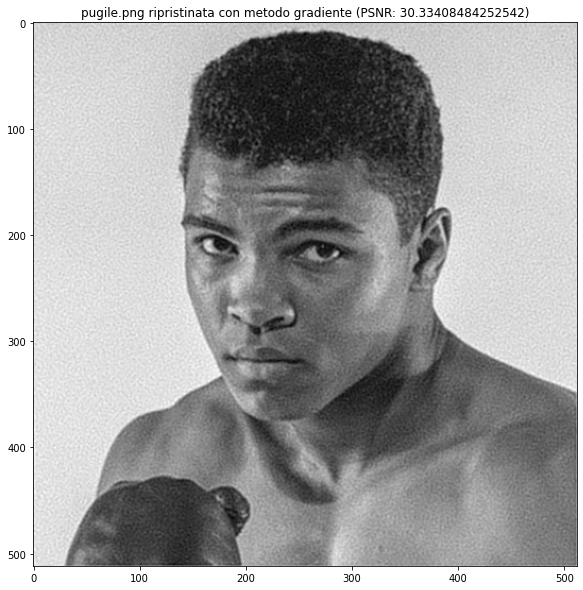
\includegraphics[width=0.6\linewidth]{imgRel/fotogrmg.png}
        \caption{Immagine fotografica ripristinata}
        \label{fig: pugilemg1}
    \end{subfigure}%
    \begin{subfigure}{0.5\textwidth}\centering
        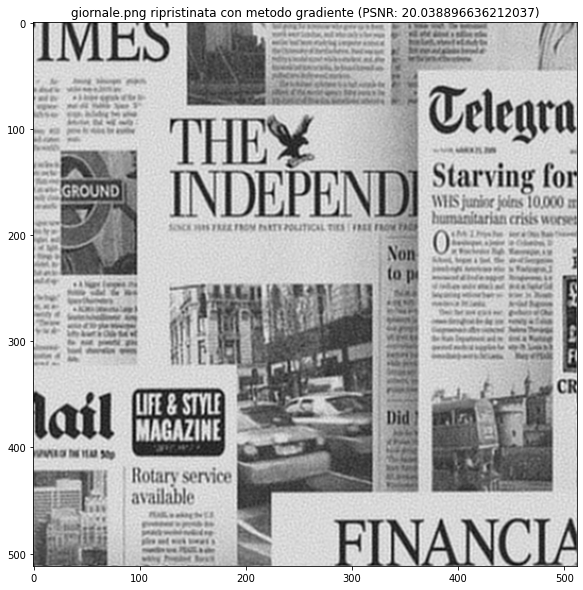
\includegraphics[width=0.6\linewidth]{imgRel/giornalemg.png}
        \caption{Immagine con testo ripristinata}
    \end{subfigure}
\caption{Immagini analizzate ripristinate con il Metodo del Gradiente}
\end{figure}
 
\begin{algorithm}[H]
	\caption{Metodo del Gradiente in \code{pseudocode}}\label{alg:mg}
	\begin{algorithmic}[1]
		\State $x_0 \in R^n, k=0$
        \While{$\nabla f(x_k) \neq 0$ and $k <$ maxit}\Comment{maxit è il massimo di iterazioni}
            \State calcolare la direzione di discesa $d_k$
            \State calcolare il passo di discesa $\alpha_k$
            \State $x_{k+1} = x_k+\alpha_kd_k$
            \State $k = k+1$
        \EndWhile
	\end{algorithmic}
\end{algorithm}

\begin{figure}[H]
    \centering
    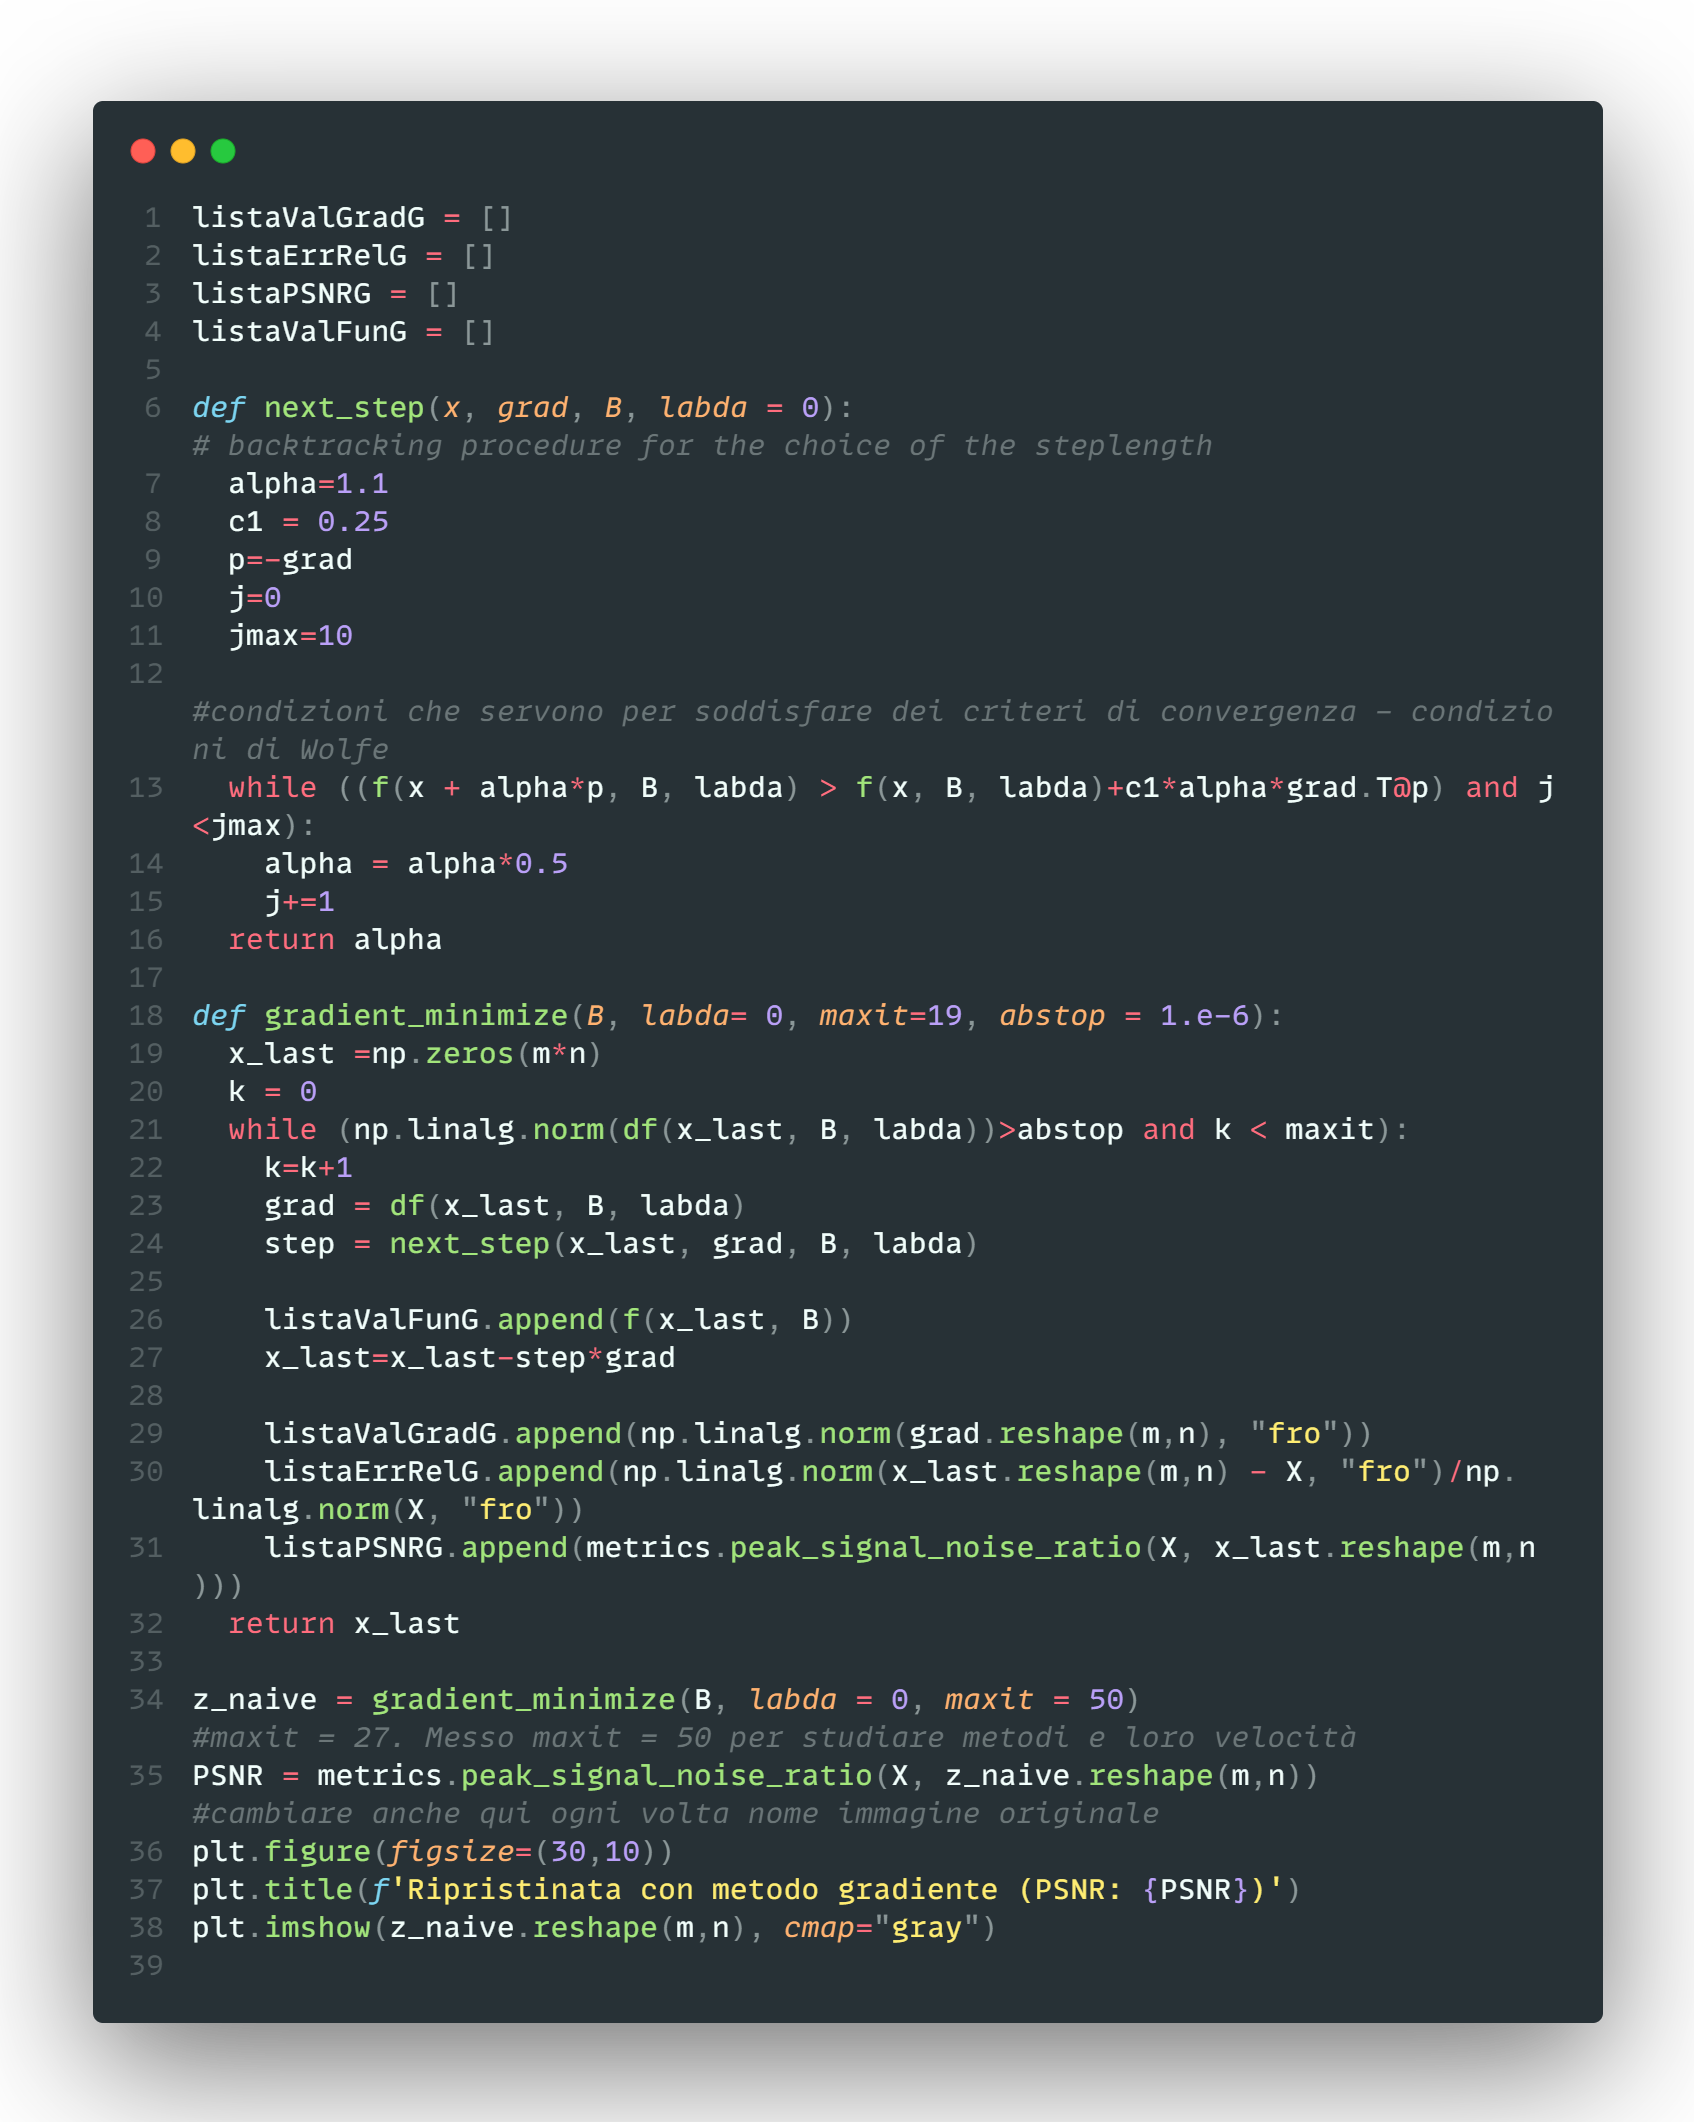
\includegraphics[width=0.7\textwidth]{imgCode/metGrad.png}
    \caption{Codice in \code{Python 3} del metodo del gradiente applicato ad una singola immagine}
\end{figure}

Notiamo anche qui che l'immagine ripristinata ha un PSNR molto piú alto rispetto all'immagine corrotta. 
Questo risulta in un'immagine con una qualità corretta e simile all'immgine originale.

Per esempio considerando l'immagine fotografica avremo che:\\
\textbf{Immagine ripristinata \ref{fig: pugilemg1}} PSNR: 30.334085\\
\textbf{Immagine corrotta \ref{fig:fotogrCorrotte7x7}} PSNR: 30.9049\\